%************************************************
\chapter{Results}\label{ch:results}
%************************************************
In this chapter, the learning performance and regularization behavior of the ALIF, STDP-ALIF, and Izhikevich neurons are compared.
Then, the effect of stacking multiple recurrent layers on the learning performance and speed is examined.
Figure \ref{fig:inoutpair} shows a typical classification result of a full validation sentence.

	\begin{figure}[ht]
	    \myfloatalign
	    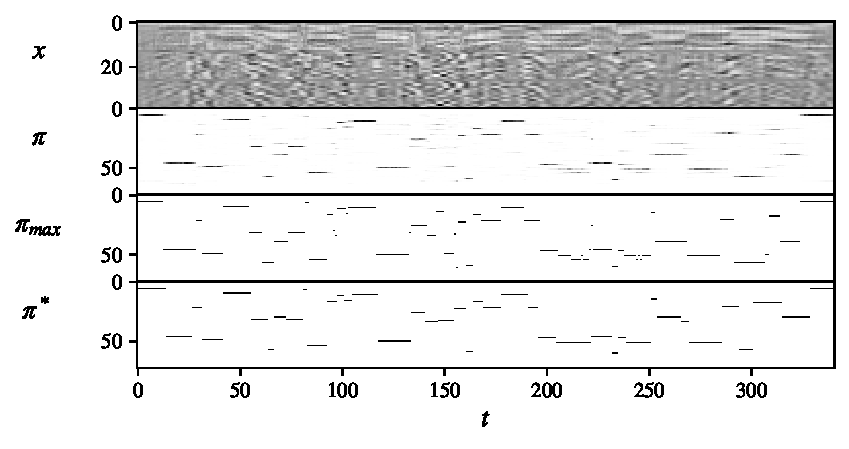
\includegraphics[width=\linewidth]{gfx/InOutPair}
	    \caption[Input-output-target example.]{An example validation result using a trained ALIF model. The top row shows the standardized MFCC frames of a sentence changing over time. The second row shows the probability distributions of the frame-wise outputs of the model. The third row is the most likely phone. The last layer shows the target phones.}
	    \label{fig:inoutpair}
	  \end{figure}

\section{Comparing neuron models}
	\paragraph{Accuracy}
		The main outcome of the neuron model comparison is that in these results, the Izhikevich neuron type performs poorly compared to the ALIF and STDP-ALIF neuron models, which reach a similar classification performance.
		In Figure \ref{fig:percwrong} the Izhikevich neuron reaches a misclassification rate of 94.2\% on the test set, which is only slightly better than constantly guessing the most frequent class.
		The ALIF neuron reaches a test misclassification rate of 50\% in relatively few iterations, and the STDP-ALIF stably reaches 50\%, and likely lower if training was continued for longer.
		Note that the test performance was obtained on the model with the best validation accuracy.

		Figure \ref{fig:crossentropy} illustrates the decrease of the cross-entropy score, which for the ALIF and STDP-ALIF neurons is comparable to that of the misclassification rate.
		The cross-entropy of the Izhikevich neuron continues to decrease while its classification accuracy stalls, suggesting that it trains its bias toward more frequent phone classes rather than learning a relationship between input MFCCs and classes.

		\begin{figure}[bth]
		    \myfloatalign
		    \subfloat[Percentage of samples wrongly classified.]
		    {\label{fig:percwrong}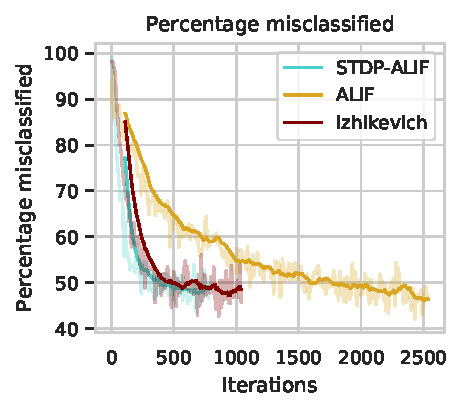
\includegraphics[height=5cm, keepaspectratio]{gfx/percwrong}} \quad
		    \subfloat[Cross-entropy loss (log-scaled).]
		    {\label{fig:crossentropy}%
		        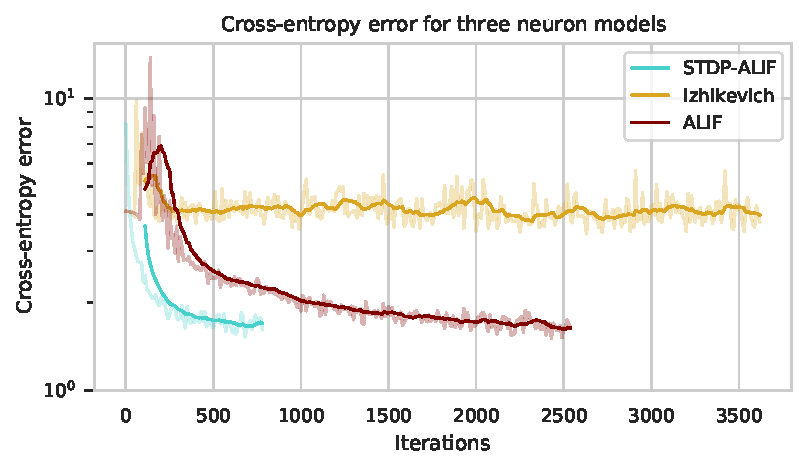
\includegraphics[height=5cm, keepaspectratio]{gfx/crossentropy}}
		    \caption[Classification performance for each of the three neuron models in a single-layer e-prop model.]{Classification performance on the validation data for each of the three neuron models in a single-layer e-prop model. The opaque lines indicate the running average of the real validation scores indicated by the transparent lines. The star symbols indicate the performances on the test set, with a misclassification rate of 92.4\% for the Izhikevich neuron, 50.3\% for the ALIF neuron, and 50\% for the STDP-ALIF neuron type.}\label{fig:sl-acc}
		\end{figure}

% testscores = {
% 	'ALIF': {1: (50.3, 1.772), 2: (64.5, 2.558), 3: (74.1, 3.345)},
% 	'STDP-ALIF': {1: (50.0, 1.751), 2: (65.3, 2.643), 3: (88.3, 4.779)},
% 	'Izhikevich': {1: (94.2, 6.794), 2: (88.2, 4.259), 3: (88.5, 4.161)}
% }

	\paragraph{Firing rate}
		Figure \ref{fig:freqs} illustrates the effect of the firing regularization term.
		It can be observed that the ALIF and STDP-ALIF neuron models are able to quickly change their mean spiking frequencies to the desired target frequency of \SI{10}{\Hz}, but the Izhikevich neuron increases past this rate to a spiking frequency of approximately \SI{18}{\Hz}.

		Figure \ref{fig:regerr} illustrates the decrease of the regularization error.
		The ALIF neuron appears to slightly better adapt to the regularization term.
		The Izhikevich neuron, again, underperforms significantly.
		\begin{figure}[bth]
		    \myfloatalign
		    \subfloat[Mean spiking frequency.]
		    {\label{fig:freqs}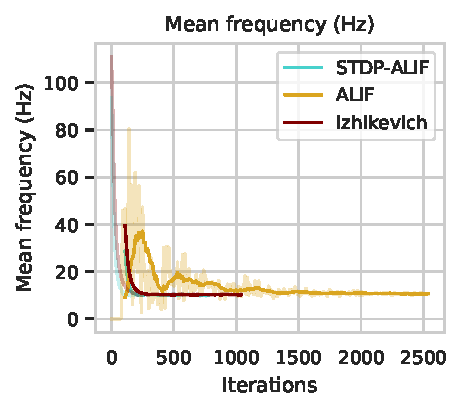
\includegraphics[height=5cm, keepaspectratio]{gfx/hz}} \quad
		    \subfloat[Regularization error.]
		    {\label{fig:regerr}%
		        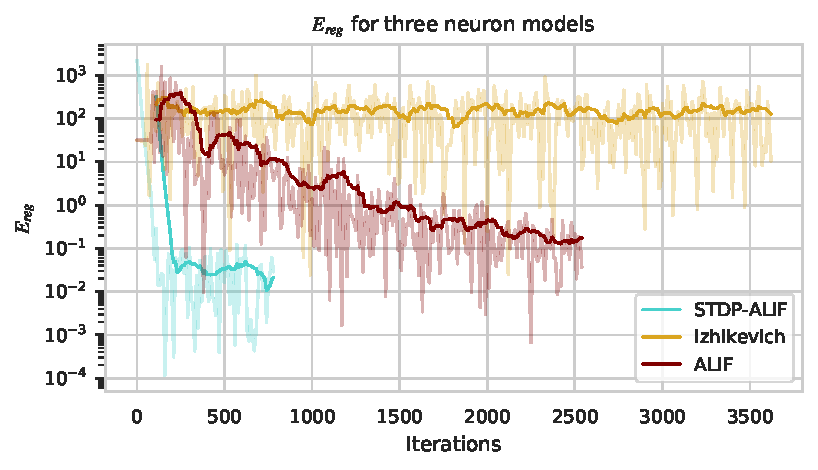
\includegraphics[height=5cm, keepaspectratio]{gfx/regerr}}
		    \caption[Effect of firing rate regularization for each of the three neuron models.]{Effect of firing rate regularization on the validation data for each of the three neuron models.}\label{fig:sl-reg}
		\end{figure}

\section{Comparing network depth}
The comparison between the network depth in Figures \ref{fig:ml-pwrong-alif}--\ref{fig:ml-pwrong-izh} suggests that single-layer e-prop networks train considerably more efficiently and accurately than multi-layer e-prop networks.
This holds for all tested neuron types.
The cross-entropy error, spiking frequency, and regularization error are also better for single-layer networks (see Figure \ref{fig:ml-otherresults}).

\begin{figure}[bth]
    \myfloatalign
    \subfloat[ALIF model.]
    {\label{fig:ml-pwrong-alif}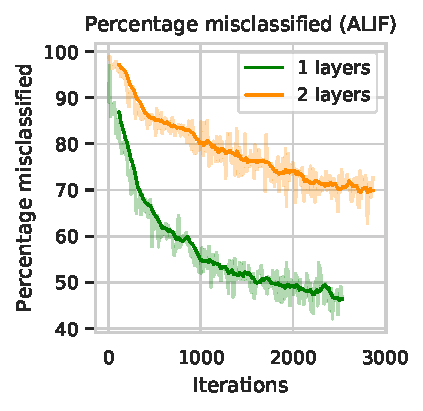
\includegraphics[height=5cm, keepaspectratio]{gfx/ml-percwrong-ALIF}} \quad
    \subfloat[STDP-ALIF model.]
    {\label{fig:ml-pwrong-stdpalif}%
        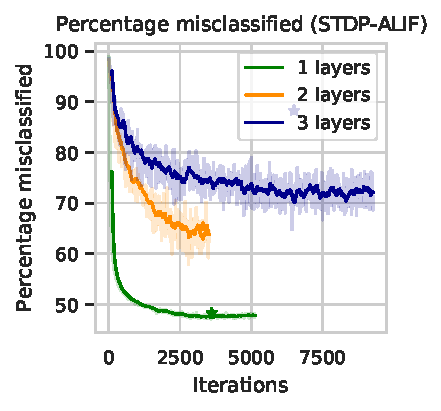
\includegraphics[height=5cm, keepaspectratio]{gfx/ml-percwrong-STDP-ALIF}} \\
    \subfloat[Izhikevich model.]
    {\label{fig:ml-pwrong-izh}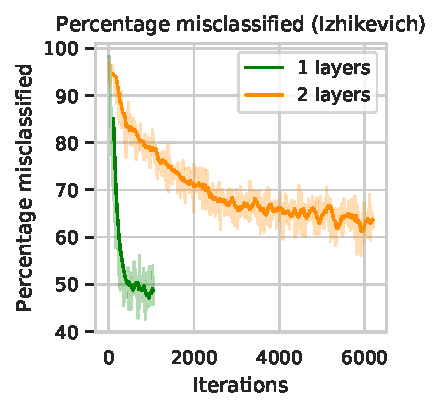
\includegraphics[height=5cm, keepaspectratio]{gfx/ml-percwrong-Izhikevich}}
    \caption[Single- and multi-layer accuracy comparison]{Accuracy comparison on the validation data between single- and multi-layer e-prop models.}\label{fig:ml-percwrong}
\end{figure}
